\section{Manual de usuario}\label{Manual usuario}

Para el correcto uso de la aplicación, el conjunto de acciones que se pueden realizar en dicho programa serán definidas a continuación. También, la distribución de las secciones de la interfaz junto a su explicación y funcionalidad.\bigskip

Cuando se ejecute el programa por primera vez en la pantalla se debe mostrar la siguiente interfaz de usuario:

\begin{figure}[!h]
    \centering
    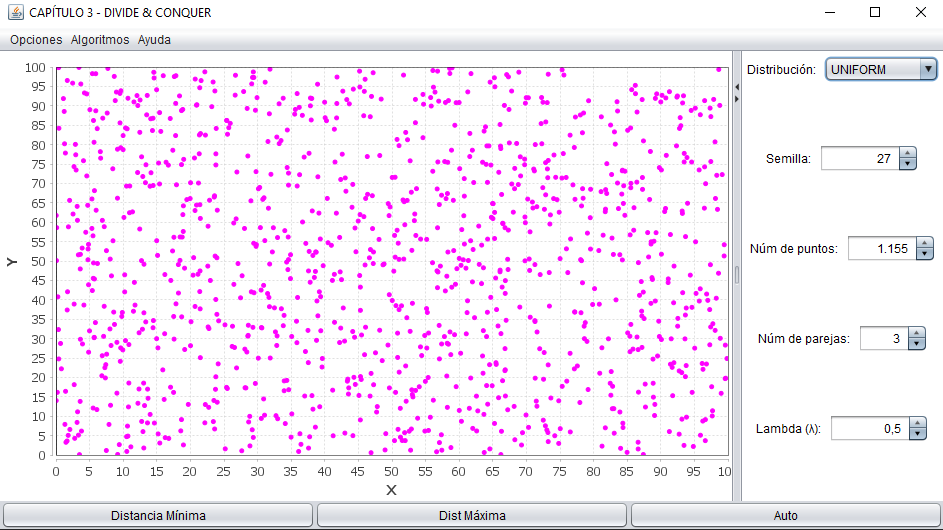
\includegraphics[width=\linewidth]{Usage/img/GUI.png}
    \caption{Interfaz de usuario}
    \label{fig:User_interface}
\end{figure}

\subsection{Menu}\label{Manual usuario, Header}

El menu de la aplicación se trata de la barra que se situa debajo del marco superior de la ventana. En esta se puede encontrar un conjunto de opciones para que el usuario pueda iteractuar con la aplicación, modificar y analizar el comportamiento de esta. En concreto, se encuentran las opciones de \say{Opciones}, \say{Algoritmos} y \say{Ayuda}.\bigskip

En la primera se situán todas las posibles acciones generales relacionadas con la aplicación, ya sea como borrar soluciones, borrar y/o resetear datos e inciar las ventanas de estadísticas explicadas anteriormente en los apartados \ref{Stats JVM} y \ref{Stats Algt}.\bigskip

En la segunda se sitúan todas las posibles acciones relacionadas directamente con la ejecución de los algoritmos, especificamente, que tipo de algoritmo ejecutar ($n^2$ y $nlogn$) y el modo de la opción auto, explicado en el apartado \ref{Footer}, ($n^2$, $nlogn$ y \say{BenchMark}).\bigskip

Y finalmente, en la última opción se encuentra un menu desplegable con un manual de usuario con la explicación del funcionamiento de la aplicación.

\subsection{Main}

El \say{Main} es el bloque principal de la vista, donde se representará gráficamente, la distribución, el número de puntos seleccionado, la semilla y la solución a los algoritmos, además de poder interactuar con el gráfico.\bigskip

\subsection{Sidebar}\label{Sidebar}

El \say{Sidebar} contiene un conjunto de opciones para modificar los datos y el modo de ejecución de la aplicación. A continuación, se explicará cada una de estas opciones y su función.\bigskip

En primer lugar, se encuentra la opción para seleccionar la \say{Distribución}. En esta, se puede escoger el tipo de distribución que queremos aplicar a la generación de puntos. En esta práctica, se han implementado las siguientes distribuciones: 
\begin{itemize}
    \item Uniform
    \item Gaussian
    \item Exponential
    \item Bernoulli
\end{itemize}
\bigskip

En segundo lugar, se halla la opción para elegir la \say{Semilla}. En esta opción, se tiene la opción cambiar el valor de la semilla para que la generación de punto se pueda replicar. Es decir, los puntos se generan aleatoriamente a partir de esta semilla.\bigskip

En tercer lugar, existe la opción para seleccionar la cantidad de puntos que se desean representar, \say{Núm. puntos}. Se podrán generar los puntos que se deseen introduciendo la cantidad en esta opción y pulsando enter. \bigskip

En cuarto lugar, se encuentra la opción para elegir el número de parejas, \say{Num. Parejas}. Esta opción permite seleccionar el número de parejas de puntos que se desea que el algoritmo encuentre. Por ejemplo, si seleccionamos 3 parejas, se calcularán 3 parejas de soluciones no repetidas. \bigskip

Por último, la etiqueta \say{Lambda}, esta solo será útil para el tipo de distribución que se haya aplicado a los puntos. La única distribución implementada la cual lambda ($\lambda$) puede contribuir a la generación de datos es la distribución Exponencial. Las demás distribuciones no se verán afectadas por lambda.

\subsection{Footer}\label{Footer}

En la sección \say{Footer}, se hallan tres botones para seleccionar el tipo de algoritmo a ejecutar.
En primer lugar, empezando por la izquierda de la interfaz, tenemos el botón Distancia mínima. Una vez el botón ha sido pulsado, se calculará la distancia mínima entre dos puntos dependiendo de los parámetros que el usuario haya introducido.\bigskip

En segundo lugar, tenemos el botón \say{Distancia máxima}. Una vez el botón ha sido pulsado, se calculará la distancia máxima entre dos puntos dependiendo de los parámetros que el usuario haya introducido.\bigskip 

Por último, el botón \say{Auto} calculará de manera repetitiva la distancia mínima o máxima entre dos puntos, a partir de los parámetros introducidos por el usuario. Se ejecutará el algoritmo seleccionado de manera iterativa hasta que se acabe el algoritmo o se pulse el botón de \say{Stop}, el cual aparece después de haber pulsado el botón \say{Auto}. Adicionalmente, esta opción permite realizar al usuario de la aplicación un \say{Benchmark} de los algoritmos de forma automática.

\subsection{Ejemplo ejecución}

Al iniciar la aplicación se mostrará una interfaz como la expuesta en la imagen \ref{fig:User_interface}. Para poder iniciar la ejecución del algoritmo, es necesario que se pulse el botón del algoritmo que se desee ejecutar, encontrar parejas a una máxima distancia o a una mínima distancia, además de seleccionar la complejidad del algoritmo que por defecto se ejecuta el $n^2$. Y, opcionalmente, modificar los datos como se ha mencionado anteriormente en la sección \ref{Sidebar}. 

A continuación, la siguiente imagen, muestra un ejemplo de la interfaz en mitad de la ejecución:

\begin{figure}[!h]
    \centering
    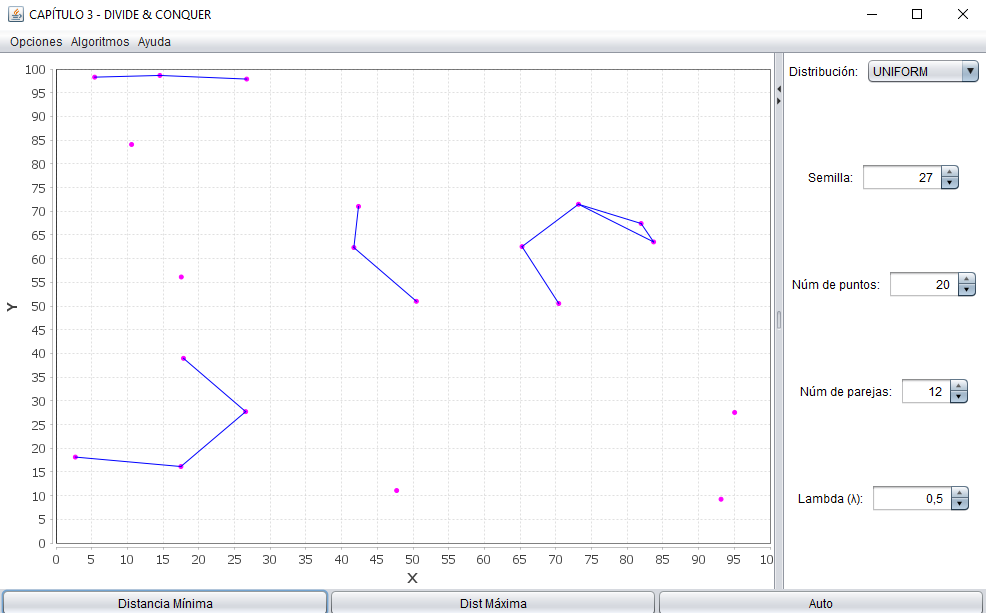
\includegraphics[width=\linewidth]{Usage/img/ejecucion.png}
    \caption{Interfaz de usuario}
    \label{fig:Ejemplo ejecución}
\end{figure}

A partir de aqui, el usuario puede reiniciar la ejecución para ejecutar nuevamente el algoritmo, borrar las soluciones obtenidas, ejecutar otros algoritmos y ver estadísticas de la ejecución, ver apartados \ref{Stats JVM} y \ref{Stats Algt}.
